\chapter*{Preface}
\markboth{Preface}{}
\addcontentsline{toc}{part}{Preface}

\paragraph{How birds fly together}
Systems far from thermal equilibrium frequently show novel features
when compared to their equilibrium counterparts. As an everyday
example, consider a group of birds displaying long-range ordered
behaviour, manifested by forming a flock under certain
conditions. This behaviour can be modeled by introducing a time step
rule, such that each individual bird in a group determines its next
direction on each time step by averaging the directions of its
neighbours and adding some random noise on top of
that~\cite{Toner1995}. It can be shown that, in the limit of the
velocity going to zero, the model reduces to the XY model in two
dimensions, where the spin is represented by the bird velocity. Since
the 2D XY model does not spontaneously break the symmetry at any
finite temperature (as justified by the Mermin-Wagner theorem), one
can show that the appearance of the long-range ordered phase is a
direct consequence of nonequilibrium aspects of the model. In a
nutshell, the neighbours of one particular bird will be different at
different times, depending on the velocity field. This gives rise to a
time-dependent variable-ranged interaction, which can stabilize the
ordered phase.

\paragraph{Driven-dissipative systems}
Non-equilibrium driven-dissipative photonic systems, such as
polaritons in semiconductor microcavities or arrays of coupled optical
resonators, have recently attracted a lot of interest due to the
possibility of observing quantum phenomena which normally require very
low temperatures and/or intense magnetic fields and are traditionally
restricted to the domain of solid-state systems or ultracold atomic
gases. Besides being highly tunable, these optical systems facilitate
direct experimental access to observables such as the wavefunction or
energy spectrum, all at room temperature. In particular, microcavity
polaritons have allowed the observation of collective hydrodynamic
phenomena, ranging from frictionless flow around a small defect to the
formation of quantized vortices and dark solitons at the surface of
large impenetrable obstacles~\cite{Carusotto_2013}, while
ring-resonator arrays coupled to artificial magnetic fields have
recently allowed engineering topological edge states robust to
disorder~\cite{hafezi2013imaging}.


\paragraph{Polaritons}
Microcavity polaritons are quasiparticles resulting from the strong
coupling of cavity photons and quantum well excitons~\cite{bastard,
  deveaud2003electron}, and have the prerogative of being both easy to
manipulate, via an external laser, and detect, via the light escaping
from the cavity~\cite{9780199228942}. The finite polariton lifetime
establishes the system as intrinsically out of equilibrium: an
external pump is needed to continuously replenish the cavity of
polaritons, that quickly, on a scale of tens of picoseconds,
escape. The pumping can be done resonantly, close to the polariton
energy dipersion, or non-resonantly.

\paragraph{Incoherent pumping: polariton BEC}
The landmark observation~\cite{Kasprzak_2006} of polariton
condensation in 2006, as shown in Fig.~\ref{fig:polBEC}, was achieved
using a non-resonant experimental setup. In the experiments, the
system was incoherently excited by a laser beam tuned at a very high
energy. Relaxation of the excess energy~\cite{RevModPhys.82.1489,
  Keeling_2007} lead to a population of the cavity polariton states
and, above a certain laser power threshold, to Bose-Einstein
condensation into the lowest polariton state.
%
\begin{figure}[tb]\centering
  \includegraphics[width=.7\linewidth]{polBEC_cond}
  \caption{
    % 
    Experimental observation of polariton Bose-Einstein
    condensation. A sharp and intense peak corresponding to the lowest
    momentum state is formed in the center of the far-field emission [top
    panels], with increasing pump power (left to right). The
    corresponding energy-resolved emission [bottom panels] show that
    above the condensation threshold, the emission comes almost entirely
    from the lowest energy state situated at the bottom of the polariton
    dispersion. From Ref.~\cite{Kasprzak_2006}.
    % 
  }\label{fig:polBEC}
\end{figure}
%

\paragraph{Coherent pumping: OPO}
Due to their energy dispersion and strong nonlinearity inherited from
the excitonic component, polaritons resonantly injected by the
external laser into the pump state with a suitable wavevector and
energy can undergo coherent stimulated scattering into two conjugate
states~\cite{Ciuti_2000,Ciuti_2001,Ciuti_2003}, called the signal and
the idler, in a process known as optical parametric oscillator
(OPO). Since their first realisation~\cite{Stevenson_2000,
  Savvidis_2000, Savvidis_2000_b, Baumberg_2000, Saba_2001}, the
interest in microcavity optical parametric phenomena has involved
several fields of fundamental and applicative
research~\cite{Edamatsu_2004, Savasta_2005, Lanco_2006, Abbarchi_2011,
  Ardizzone_2012, Xie_2012, Lecomte_2013}. 

%
\begin{figure}[tb]\centering
  \includegraphics[width=.8\linewidth]{hafezi}
  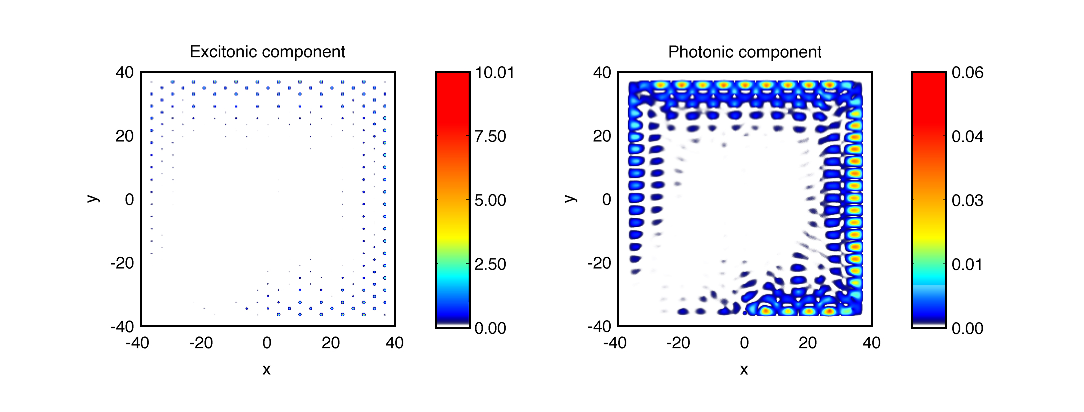
\includegraphics[width=.8\linewidth]{polaritopo}
  \caption{
    % 
    \emph{Top panels:} Simulated (right panel) and observed (left panel)
    edge state propagation in a ring-resonator array.  The light enters
    from one corner and exits from the other, as signaled by the
    arrows. Adapted from Ref.~\cite{hafezi2013imaging}.  \emph{Bottom
      panels:} Simulated edge state propagation in a polariton system.
    Intensities of the exciton (left panel) and photon (right panel)
    fields obtained when pumping a lattice at the center of its lower
    edge. From Ref.~\cite{PhysRevX.5.031001}.
    % 
  }\label{fig:topolariton}
\end{figure}
%
\paragraph{Superfluidity}
The superfluid properties of a resonantly pumped polariton quantum
fluid, both in the pump-only configuration (without parametric
scattering) as well as the OPO regime, have been actively investigated
experimentally, as well as theoretically~\cite{Carusotto_2013}. In
particular, a supression of scattering in the pump-only case was
observed~\cite{Amo_2009} below a critical velocity, similar to what
has been predicted by the Landau criterion for equilibrium superfluid
condensates.
%
While in equilibrium condensates different aspects of superfluidity
are typically closely related~\cite{Leggett_1999}, this is no longer
true in a non-equilibrium context.  Independent of the pumping scheme,
the driving and the polariton finite lifetime force one to reconsider
the meaning of superfluid behaviour, when the spectrum of collective
excitations is complex rather than real, raising question about the
applicability of a Landau criterion~\cite{Wouters_2010}.
%
An additional complexity characterises the OPO regime, namely, the
simultaneous presence of three oscillation frequencies and momenta for
pump, signal and idler correspondingly increases up to 12 (or 6,
depending on the approximation used to describe the system) the number
of collective excitation branches~\cite{Wouters_2007}. Note that from
the experimental point of view, pioneering
experiments~\cite{Amo_2009_b} have observed a ballistic nonspreading
propagation of signal/idler polariton wavepackets in a triggered-OPO
configuration, as well as demonstrating the existence and
metastability of vortex configurations~\cite{Sanvitto_2010} in the
signal and idler.
 

\paragraph{Topology in polaritons}
Very recently, the polariton community started to explore topological
effects in polariton lattices~\cite{PhysRevB.93.020502,
  PhysRevB.91.161413, PhysRevLett.114.116401, PhysRevB.93.085438,
  PhysRevX.5.031001}. The idea is to break time reversal symmetry by
the application of a strong external magnetic field, giving rise to
energy bands with nontrivial topology. In particular,
Ref.~\cite{PhysRevX.5.031001} proposes an exciton-photon coupling with
a winding phase in momentum space, giving rise to polaritonic bands
with chiral edge modes that allow unidirectional propagation,
protected against backscattering. The bottom panels of
Fig.~\ref{fig:topolariton} show the exciton and photon fields
traveling together as a unique polaritonic counter-clockwise chiral
edge mode. In this context, dissipation in the form of photon losses
provides a coupling to the outside continuum of modes and, as such,
can be used to detect or inject edge modes.
%
It would be interesting to study the feasability of coupled
micropillars for this type of physics, in view of the recent
experimental findings of a linear graphene-like
dispersion~\cite{Jacqmin_2014} as well as edge
states~\cite{polaritonedge} in honeycomb micropillar lattices.  
%
On the other hand, topologically protected edge states have already
been experimentaly observed~\cite{hafezi2013imaging} in the case of
silicon-based optical resonator arrays (see top panels of
Fig.~\ref{fig:topolariton}), due to recent advances in creating
synthetic gauge fields, which have opened new horizons for simulating
topological phases of matter also with neutral particles, such as
photons~\cite{hafezi2014synthetic} (or ultracold
atoms~\cite{dalibardrmp2011, goldman_repprog_2014,
  Goldman_arxiv_2015}). Rather than simply replicating previous
measurements, experiments with synthetic gauge fields allow for
unprecedented access to properties such as the eigenstates or
eigenspectrum, while the tunability and controllability of these
experiments offer the prospect of simulating novel physics.


\subsection*{Contents of this thesis}
\paragraph{Thesis layout}
This manuscript is split in two parts: part I is a detailed review of
the basic concepts, including both the theoretical formalism, as well
as the relevant experiments, necessary for understanding part II,
which presents the three main works published as part of my PhD
(Chapters~\ref{cha:drag},~\ref{cha:opo} and~\ref{cha:landau}). The two
systems chosen for ilustrating the basic physical concepts are
ultracold atomic gases (Chapter~\ref{cha:cold-gases}) and microcavity
exciton-polaritons (Chapter~\ref{cha:polaritons}). We now give a brief
description of the content of each of the chapters.

In Chapter~\ref{cha:cold-gases}, we describe the phenomenon of
Bose-Einstein condensation, and introduce the Gross-Pitaevskii
equation which is extended in Chapter~\ref{cha:polaritons} to the case
of polariton condensates. We then review the linear response of a
moving atomic condensate to a weak stationary defect, leading to
discussion on superfluidity. This scattering problem is the
equilibrium conterpart of the problems studied in
Chapters~\ref{cha:drag} and~\ref{cha:opo} in the context of polaritons
in the resonantly pumped and optical parametric oscillator regimes,
respectively. Finally, we introduce the Harper-Hofstadter model, which
is the backbone of Chapter~\ref{cha:landau}.

In Chapter~\ref{cha:polaritons}, we introduce microcavity
exciton-polaritons, and their theoretical description in terms of a
driven-dissipative Gross-Pitaevskii equation. We discuss both the
resonantly pumped system which is used in Chapter~\ref{cha:drag}, as
well as the optical parametric oscillator of Chapter~\ref{cha:opo},
and we make the connection to the superfluid-related phenomena
previously introduced in Chapter~\ref{cha:cold-gases}.

In Chapter~\ref{cha:drag}, we study the scattering of a resonantly
pumped polariton condensate against a static defect of the
microcavity, for the simplified case of small fluid velocities, when
the polariton dispersion can be considered quadratic. After discussing
the effects of dissipation on the Bogoliubov excitation spectra, we
find that the finite polariton lifetime also affects the drag exerted
by the condensate on the defect. In particular, we show that there is
a nonzero drag force, entirely due to the out-of-equilibrium nature of
the system, even in the ``superfluid regime''. Finally, we
characterise the behaviour of the drag as a function of the condensate
velocity and polariton lifetime.

In Chapter~\ref{cha:opo}, we present a theoretical and experimental
study of the same scattering problem, now in the context of an optical
parametric oscillator consisting of three coupled condensates: the
pump, the signal and the idler. Apart from using the linear response
analysis first introduced in Chapter~\ref{cha:cold-gases} and then
extended to the case of a pump-only condensate in
Chapter~\ref{cha:drag}, we also numerically solve the full
driven-dissipative Gross-Pitaevskii equation. We show that, while the
modulation patterns are present in all three condensates, their
relative amplitudes depend on various factors. In particular, for the
typical experimental conditions that favour parametric scattering, the
signal has undetectable modulations, while the pump and idler show the
same response.

In Chapter~\ref{cha:landau}, we add a harmonic trap to the
Harper-Hofstadter lattice model of Chapter~\ref{cha:cold-gases}. We
discuss how the eigenstates of the new Hamiltonian can be seen as
momentum-space Landau levels, by making use of the nontrivial topology
of the Harper-Hofstadter energy bands. We then extend the model to
include driving and dissipation, and finally present a proposal for
the physical implementation of the model in state-of-the-art
driven-dissipative photonic systems.

The source code belonging to Chapters~\ref{cha:drag},~\ref{cha:opo}
and~\ref{cha:landau} is available online~\cite{SourceCode}.


%%% Local Variables:
%%% mode: latex
%%% TeX-master: "../thesis_berceanu"
%%% End:
